% Packages utilisés~: fontenc, geometry, indentfirst, marvosym, esvect, wrapfig, physics, amssymb, mathtools, mhchem (v4), chemfig, adjustbox, enumitem, rsfso, cancel, makecell, subcaption, multicol, tikz, fancyhdr, lastpage, siunitx, tcolorbox, ifthen, caption, multirow, float.


\documentclass{article}
\usepackage[T1]{fontenc}
\usepackage[a4paper, margin=2cm]{geometry}
\usepackage{indentfirst} %indente qu'après un titre
\usepackage{marvosym} %symbol de la main qui écrit
\usepackage{esvect} %jolis vecteurs
\usepackage{wrapfig} %figures wrapped
\usepackage{physics} % macros de Physique
\usepackage{amssymb} % Symboles de Maths
\usepackage{mathtools} % Maths
\usepackage[version=4]{mhchem} % écrire des formules de chimie plus facilement
\usepackage{chemfig} % traçage de molécules
\usepackage{adjustbox} % pour les tableaux trop larges
\usepackage{enumitem} % pour garder un itemize et la ligne qui précède
\usepackage[scaled=1.1,scr]{rsfso} %pour les fontes scr 
\usepackage[makeroom]{cancel} %barrer des choses en diagonale (e.g. C2 §VIII.7)
\usepackage{makecell} %cases de tableau de plusieurs lignes
\usepackage{subcaption} %mettre deux figures à côté
\usepackage{multicol}

% TikZ
\usepackage{tikz} % Outil de dessin TikZ
\usetikzlibrary{positioning, decorations, decorations.pathmorphing, svg.path, calc}
\usepackage{pgfplots}
\pgfplotsset{compat=1.17}


\newcommand{\serpeg}{
\begin{tikzpicture}[scale=0.05, rotate=90] %Dessin serpe gauloise
    \draw[fill=black] svg "m 85.80084559909016,214.0848263194619 -2.06515398583127,10.6699622601283 C 63.40206828227082,245.1959395037747 34.8434652071972,311.9906290729065 11.3692540264214,288.5164178921307 -12.10495715435405,265.0422067113552 54.64670837340594,236.4405795949098 75.08785929759045,216.1069562639218 l 10.71298630149971,-2.0221299444599 z";
    \draw[fill=black] svg "m 108.7419167440706,206.736972338917 -19.8340830722545,19.8340830722545 c 1.52410126960524,2.0394970349658 1.73127876250413,4.4641831949897 0.38721637234333,5.8082455851505 -1.5360713030409,1.536071303041 -4.54941029245121,1.0437150858417 -6.71175045395158,-1.1186250756586 L 68.55746210310377,217.2348384335593 c -2.16234016150031,-2.1623401615003 -2.61167233732806,-5.1326551095392 -1.07560103428716,-6.6687264125801 1.34406239016084,-1.3440623901608 3.76874855018474,-1.1368848972619 5.80824558515053,0.3872163723434 l 19.83408307225447,-19.8340830722546 15.61772701784898,15.617727017849 z";
    \draw[fill=black] svg "m 235.6535816959719,31.9640591939666 c 43.897708386389,43.897708386389 43.8977083863892,115.0331004398762 0,158.930808826265 -43.7245047247137,43.724504724714 -114.4767693137891,43.8957526893702 -158.41452032980723,0.5162884964578 l 16.95147230036508,-20.5654917755697 c 38.81906059246856,27.569114427687 92.07923865044546,24.7740577145076 125.80229697022164,-8.9490006052689 C 257.7671841813877,124.1223105912145 256.7199821471888,61.89341216770936 217.6695324026912,22.84296242321181 211.1465363002555,16.3199663207761 203.9694091953853,10.84862686886356 196.3726319238062,6.450802660676091 210.6929035158315,11.9233868411129 224.1124996231,20.42297712109476 235.6535816959719,31.9640591939666 z";
\end{tikzpicture}}

\newcommand{\nez}{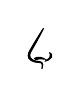
\begin{tikzpicture}[scale=0.0015] %Dessin sens Physique
    \draw[fill=black] svg "M5613.5,4620.6C4873.8,3491.5,3821,1773.4,2823,69c-547.9-935.4-655.5-1207.4-655.5-1673.1c0-238.7,35.2-403.1,117.4-571.4c240.7-483.3,771-821.9,1540-982.3c324.8-66.5,526.4-90,964.7-107.6c332.7-11.7,391.4-19.6,461.8-56.7c107.6-54.8,189.8-152.6,244.6-291.6c43-103.7,47-140.9,45-455.9c0-272-9.8-381.6-41.1-528.3c-23.5-101.8-39.1-189.8-35.2-191.8c3.9-3.9,33.3,74.4,64.6,176.1c209.4,653.6,176.1,1129.1-97.8,1375.7c-135,121.3-264.2,164.4-569.4,187.9c-630.1,47-1164.3,172.2-1569.4,367.9c-628.1,305.3-886.4,753.4-763.2,1326.7c64.6,311.1,129.2,444.2,649.7,1356.1C4143.9,1691.2,4893.3,3061,5525.4,4295.8c303.3,591,364,714.2,352.2,714.2C5873.7,5010,5754.4,4833.9,5613.5,4620.6z";
    \draw[fill=black] svg "M7407.9-968.2c-3.9-5.9,7.8-72.4,29.4-150.7c86.1-332.7,60.7-731.8-62.6-947.1c-68.5-115.5-236.8-293.5-405-422.7c-125.2-95.9-428.6-285.7-546-342.4c-70.4-33.3-90-64.6-39.1-64.6c58.7,0,495.1,154.6,636,225c342.5,172.2,596.8,401.2,739.7,665.3c70.5,133.1,72.4,142.9,72.4,342.5s-1.9,213.3-74.4,356.2C7664.2-1114.9,7458.8-917.3,7407.9-968.2z";
    \draw[fill=black] svg "M4261.3-2026.8c-164.4-35.2-471.6-185.9-536.2-264.2c-109.6-129.2-43.1-197.7,232.9-242.7c219.2-35.2,250.5-31.3,471.6,58.7c86.1,37.2,230.9,76.3,320.9,90c211.3,29.3,645.8,13.7,1074.3-41.1c174.2-23.5,322.9-37.2,328.8-31.3c62.6,62.6-634,340.5-1056.7,420.7C4848.3-1987.7,4460.9-1983.8,4261.3-2026.8z";
\end{tikzpicture}}


% Pied de page et en-tête
\usepackage{fancyhdr}
\usepackage{lastpage}

% Style de première page (sans header)
\fancypagestyle{plainsh}{
    \fancyhf{}%
    \renewcommand{\headrulewidth}{0.0pt}
    \cfoot{\footnotesize Page \textbf{\thepage}\ sur \textbf{\pageref{LastPage}}}
}

% style général
\makeatletter
\fancypagestyle{plain}{
    \fancyhf{}%
    \setlength{\headheight}{14.0pt} 
    \fancyhead[R]{\large{\acronyme{} -- \@title}}
    \fancyhead[L]{\large{MP1, 2021-2022}}
    \cfoot{\footnotesize Page \textbf{\thepage}\ sur \textbf{\pageref{LastPage}}}
}
\makeatother

% choix du style général
\pagestyle{plain}


%titres
\renewcommand{\abstractname}{Introduction}
\usepackage{sectsty}
\renewcommand{\thesection}{\Roman{section}.}
\renewcommand{\thesubsection}{\thesection\ \arabic{subsection})}
\renewcommand{\thesubsubsection}{\thesection\ \arabic{subsection})\ \alph{subsubsection})}

%Définition de la taille \HUGE
\usepackage{fix-cm}
\makeatletter
\newcommand\HUGE{\@setfontsize\Huge{50}{60}} 
\makeatother

% Personnalisation du titre
\makeatletter
\renewcommand\maketitle{
    \allsectionsfont{\sffamily}
    \thispagestyle{plainsh}
    \vspace*{2cm}
    \begin{center}
        \begin{minipage}{0.1\linewidth}   
            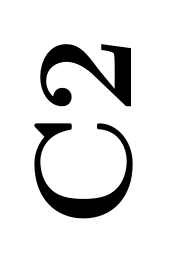
\begin{tikzpicture}
                \node [rotate=90] {\HUGE\textbf{\acronyme}}; % Référence du chapitre
            \end{tikzpicture}
        \end{minipage}
        \hspace{0.5em}
        \begin{minipage}{0.8\linewidth}
            {\raggedright
            {\Huge \bfseries \sffamily \@title }\\[1ex] 
            {\Large  \@author}\\[4ex]}  
        \end{minipage}
    \end{center}
    \vspace{0.5cm}
}
\makeatother

% package pour les unités SI
\usepackage[load-configurations = abbreviations]{siunitx}
\sisetup{locale=FR, inter-unit-product=\ensuremath{{\cdot}}, detect-all, retain-explicit-plus}
\DeclareSIUnit{\ions}{\mathrm{ions}}

% cases

\usepackage{tcolorbox} %Pour les boxes de coleur
\tcbuselibrary{skins, breakable}
\usepackage{ifthen} % algorithmique

\definecolor{lav}{HTML}{800080}
\newtcolorbox{enonce}[1][]{%
    enhanced, attach boxed title to top left=
{xshift=-2mm,yshift=-2mm}, boxed title style={size=small,colback=blue!80}, breakable,colframe=blue!80,colback=blue!10, title={#1}
}

\newtcolorbox{remarque}[1][]{%
    enhanced, attach boxed title to top left=
{xshift=-2mm,yshift=-2mm}, boxed title style={size=small,colback=lav}, breakable,colframe=lav,colback=lav!10, title={#1}
}

\newtcolorbox{important}[1][]{%
    enhanced, attach boxed title to top left=
{xshift=-2mm,yshift=-2mm}, boxed title style={size=small,colback=red!75}, breakable,colframe=red!75,colback=red!10, title={#1}
}

% Types d'écrits
\newtcolorbox{tableau}[1][]{% %ce qu'il faut recopier au tableau
    grow to left by=0.5cm, enhanced, frame hidden, left=1.25cm, right=0cm, borderline west = {0.5pt}{1cm}{red, dashed}, colback=white, breakable, segmentation style={}, overlay={%
        \ifthenelse{\value{tcbbreakpart}=1}{% seulement pour le premier morceau
            \begin{tcbclipframe}
                \coordinate (X) at ([xshift=5mm,yshift=-5mm]frame.north west);
                \node[inner sep=1mm, color=black, font=\bfseries] at (X) {\LARGE{\WritingHand}};
            \end{tcbclipframe}
        }{}
    }
}

\newtcolorbox{appnum}[1][]{% %application numérique
    grow to left by=0.5cm, enhanced, frame hidden, left=1.25cm, right=0cm, borderline west = {0.4pt}{1cm}{red, decoration = {zigzag, segment length = 2mm, amplitude = 0.4mm}}, opacityfill=0, breakable, segmentation style={} , overlay={%
        \ifthenelse{\value{tcbbreakpart}=1}{% seulement pour le premier morceau
            \begin{tcbclipframe}
                \coordinate (X) at ([xshift=5mm,yshift=-5mm]frame.north west);
                \node[inner sep=1mm, color=black, font=\bfseries] at (X) {\serpeg};
            \end{tcbclipframe}
        }{}
    }
}

\newtcolorbox{sensphy}[1][]{% %Discussion physique~!
    grow to left by=0.5cm, enhanced, frame hidden, left=1.25cm, right=0cm, borderline west = {0.8pt}{1cm}{red, dotted}, opacityfill=0, breakable, segmentation style={} , overlay={%
        \ifthenelse{\value{tcbbreakpart}=1}{% seulement pour le premier morceau
            \begin{tcbclipframe}
                \coordinate (X) at ([xshift=5mm,yshift=-5mm]frame.north west);
                \node[inner sep=1mm, color=black, font=\bfseries] at (X) {\nez};
            \end{tcbclipframe}
        }{}
    }
}

\newtcolorbox{attention}[1][]{%
    grow to left by=0.5cm, enhanced, frame hidden, left=1.25cm, right=0cm, borderline west = {0.5pt}{1cm}{red}, opacityfill=0, breakable, segmentation style={} , overlay={%
        \ifthenelse{\value{tcbbreakpart}=1}{% seulement pour le premier morceau
            \begin{tcbclipframe}
                \coordinate (X) at ([xshift=5mm,yshift=-5mm]frame.north west);
                \node[inner sep=1mm, color=black, font=\bfseries] at (X) {\large{\fontencoding{U}\fontfamily{futs}\selectfont\char 66\relax}};
            \end{tcbclipframe}
        }{}
    }
}

\newenvironment{Figure}
  {\par\medskip\noindent\minipage{\linewidth}}
  {\endminipage\par\medskip}


% esthétique
\let\oldref\ref
\renewcommand{\ref}[1]{(\oldref{#1})}
\newcommand{\ds}{\displaystyle}
\usepackage{caption}
\usepackage{multirow}
\newcommand{\Dr}{\Delta_{\mathrm{r}}}
\newcommand{\Df}{\Delta_{\mathrm{f}}}
\renewcommand{\arraystretch}{1.5} % change la hauteur des cases des tableaux
\usepackage{float}


% commandes corps de texte
\newcommand{\ext}{\text{ext}}
\newcommand{\cste}{\text{cste}}
\newcommand{\EI}{\mathrm{EI}}
\newcommand{\EF}{\mathrm{EF}}
\newcommand{\rev}{\text{rév}}
\newcommand{\fp}{{\substack{\text{forces}\\\mathclap{\text{pressantes}}}}}
\newcommand{\pg}{\substack{\text{phase}\\\text{gazeuse}}}
\newcommand{\tprod}{\text{prod}}
\newcommand{\creee}{\text{créée}}
\renewcommand{\th}{\mathrm{th}}
\newcommand{\echangee}{\text{échangée}}
\newcommand{\Tz}{T_0 = \SI{298}{K}}
\newcommand{\Pz}{P^\circ = \SI{1,00}{bar}}
\newcommand{\cz}{c^\circ = \SI{1,00}{\mole\per\liter}}
\newcommand{\albe}{{\alpha \rightarrow \beta}}

\title{Applications du second principe à la transformation chimique}
\newcommand{\acronyme}{C2}
\author{Guillaume \textsc{Saget},\\Professeur de Sciences Physiques au Lycée Champollion}

% Pour gérer la version support de cours et version entière
\newboolean{support}
\setboolean{support}{false} %changer sur true pour remplacer toutes les parties du tableau par "à faire"

\ifthenelse{\boolean{support}}
{\renewenvironment{tableau}
    {\begin{center}
        \textbf{À faire}
    \end{center}\comment}
    {\endcomment}}
{}

\begin{document}

\maketitle
\begin{abstract}
    Ce chapitre est consacré à l'étude des transformations chimiques d'un point de vue de la thermodynamique (branche de la chimie appelée thermochimie). Le premier chapitre était consacré au Premier principe qui est un principe de conservation de l'énergie. Cependant, il n'est pas capable de prédire dans quels sens se font les transferts thermiques. Il faut, pour ce faire, avoir recours au Second principe de la Thermodynamique et l'introduction de l'entropie $S$. Ceci dit, l'étude du sens d'évolution des transformations chimiques par le seul emploi de l'entropie n'est pas satisfaisant~: il faut avoir recours à une fonction thermodynamique ayant les propriétés ad hoc~: \textbf{un potentiel thermodynamique}. En outre, les transformations chimiques étant pour la plupart monobares et monothermes, le potentiel thermodynamique qui convient est $G^*$. Nous verrons que ses variations coïncident avec celles de la fonction de Josiah Gibbs ou enthalpie libre $G$ (fonction d'état adaptée aux variables d'état intensives $T$ et $P$)~: l'enthalpie libre est in fine le potentiel thermodynamique de la thermochimie. La Thermochimie d'évolution s'est construite autour d'un vocabulaire spécifique~: \textbf{le potentiel chimique}.
\end{abstract}

\section{Rappels de Thermodynamique classique concernant le second principe}
\subsection{Énoncé heuristique de R. Clausius}
Dans le deuxième principe énoncé par Carnot\footnote{Nicolas Léonard Sadi Carnot (1796 - 1832), physicien français~; il a la paternité du premier énoncé du Second Principe de la thermodynamique en 1824. Le second Principe a donc été énoncé 25 ans avant le Premier~! Le Troisième le sera 90 ans plus tard par Walter Nernst bien que la formulation «~taupinale~» soit, en fait, due à Max Planck...}, Clausius\footnote{Rudolf Clausius (Koszalin, 1822 - Bonn, 1888)~: physicien allemand. On lui doit en Thermodynamique le fameux théorème du viriel (voir Module Navale et/ou TS2) et l'un des premiers calculs de la pression cinétique.} et Thomson\footnote{William Thomson, anobli Lord Kelvin of Largs (1824, Irlande - 1907), physicien britannique véritable prodige de la physique.}, on introduit une grandeur non conservative~: l'entropie dont la production est directement liée au sens d'écoulement du temps.

\begin{enonce}[Énoncé heuristique]
    Il existe une fonction d'état extensive $S$\footnotemark{} appelée \textit{entropie}. La variation d'entropie de l'univers ne peut qu'augmenter.
\end{enonce}
\footnotetext{La notion d'entropie a été introduite par Clausius en 1865.}

\subsection{Mise en forme}
\begin{tableau}
    \textit{Univers}~: Système fermé $\Sigma$ et thermostat à la température $T_0$. L'univers est isolé.\\
    
    En notant $Q$ et $Q_\th$ les transferts thermiques (algébriques) reçus par $\Sigma$ et par le thermostat, on a $Q+Q_\th = 0$ car le système est isolé.\\
    
    Au cours d'une transformation finie, d'après l'énoncé de Clausius, $\Delta S_{\text{univers}} \geq 0$. Or, $S$ est une fonction additive donc $\Delta S_{\text{univers}} = \Delta S_\Sigma + \Delta S_{\text{thermostat}} \geq 0$.
    
    \begin{enonce}[Première identité de la Thermodynamique]
        Pour une transformation élémentaire~:
        \begin{equation}\label{id1th}
            \dd{U} = T\dd{S} - P\dd{V}
        \end{equation}
    \end{enonce}
    
    Appliquons \ref{id1th} au thermostat. On rappelle que pour un thermostat, les transferts thermiques se font sans variation de volume (Cf. MPSI). On a~:
    \begin{align*}
        \dd{U_\th} &= T_0\dd{S_\th}\qquad (\dd{V_\th} = 0)\\
        \implies \dd{S_\th} &= \frac{\dd{U_\th}}{T_0}
    \end{align*}
    
    Appliquons le premier principe entre $t$ et $t+\dd{t}$~:
    $$\dd{U_\th} = \delta W_{\fp} + \delta Q_\th$$
    
    On obtient donc~:
    \begin{align}
        \Delta U_\th &= Q_\th = -Q \implies \Delta S_\th = \frac{\Delta U_\th}{T_0} = \frac{-Q}{T_0} \nonumber \\
        \text{D'où,}\quad \Delta S_{\text{univers}} &= \Delta S_\Sigma + \Delta S_\th \geq 0 \implies \Delta S_\Sigma \geq \frac{Q}{T_0} \label{inegclau}
    \end{align}
    On peut réécrire \ref{inegclau} sous la forme~:
    $$\Delta S_\Sigma = \underbrace{\frac{Q}{T_0}}_{\mathclap{S_\echangee}} + \underbrace{S_{\begin{subarray}{l}\text{production}\\\text{ou créée}\end{subarray}}}_{\geq 0}$$
    Et,
    \begin{itemize}
        \item $S_\creee > 0$ si la transformation est irréversible~;
        \item $S_\creee = 0$ si la transformation est réversible.
    \end{itemize}
\end{tableau}

\subsection{Énoncé}
\begin{tableau}
    \begin{enonce}[Énoncé]
        Soit un système fermé $\Sigma$ (système n'échangeant pas de matière avec l'extérieur). Il existe une fonction d'état extensive appelée \textit{entropie} $S$~; lors d'une transformation élémentaire monotherme, la variation d'entropie du système est~:
        $$\dd{S_\Sigma} = \underbrace{\frac{\delta Q}{T_0}}_{\mathclap{\delta S_\echangee}} + \underbrace{\delta S_\tprod}_{\geq 0}$$
    \end{enonce}
    Où~:\nobreak
    \begin{itemize}[beginpenalty=10000] % Empêche le changement de page juste avant la liste
        \item $\frac{\delta Q}{T_0}$ désigne la variation élémentaire d'entropie reçue algébriquement par le système~;
        \item $\delta S_\tprod$ l'entropie élémentaire de production ou entropie créée qui ne peut être que positive ou nulle (transformation réversible).
    \end{itemize}
    \tcbline
    \textbf{Cas particulier~: transformation réversible}\\
    Tout au long de cette transformation, les équilibres mécaniques et thermiques sont assurés~: $T=T_0,\ P=P_\ext$. On a~:
    $$\dd{S_\Sigma} = \frac{\delta Q}{T_0} + \underbrace{\delta S_\tprod}_{= 0} = \frac{\delta Q}{T_0}$$
\end{tableau}

\section{Les potentiels thermodynamiques}
\subsection{Position du problème}
Les paragraphes \textsf{II.} à \textsf{IV.} sont des compléments de Thermodynamique classique. Tous les systèmes mis en jeu sont des systèmes fermés qui ne sont le siège d'aucune transformation chimique. La prise en compte des \textbf{transformations chimiques relève de l'étude des paragraphes \textsf{V.}} \textit{et sequentes}.

\subsection{Définition}
\begin{enonce}
    On appelle \textit{potentiel thermodynamique} $G^*$ (grandeur homogène à une énergie~; unité SI~: le joule) une fonction dépendant des variables d'état du système ($P$, $T$, $V$, etc...) \textbf{et} des paramètres extérieurs liés aux contraintes de l'évolution\footnotemark{}.
\end{enonce}
\footnotetext{Ce n'est donc pas une fonction d'état~!}

\subsection{Propriétés fondamentales}
Un potentiel thermodynamique possède les propriétés suivantes~:
\begin{itemize}
    \item Il est minimal (par rapport aux variables d'état dont il dépend) lorsque l'état d'équilibre thermodynamique du système est atteint~;
    \item Il ne peut que diminuer lorsque le système est en évolution\footnotemark{}.
\end{itemize}
\footnotetext{\begin{attention} Une transformation relie deux états d'équilibre du système. Une évolution relie  l'état d'équilibre initial à un état final dont on recherche les conditions via le potentiel thermodynamique \textit{ad hoc} pour qu'il corresponde à un état d'équilibre. \end{attention}}

\begin{important}
    Le comportement des potentiels thermodynamiques nécessite d'invoquer les deux principes de la thermodynamique.
\end{important}

\begin{remarque}[Remarque]
    Les potentiels thermodynamiques permettent de déterminer le sens d'évolution des variables d'état du système sans indication cependant de la vitesse à laquelle les ajustements aux contraintes s'effectuent.
\end{remarque}

\section{Le potentiel thermodynamique $G^*$, potentiel adapté à une évolution monotherme et monobare}
\subsection{Hypothèses de travail du paragraphe \textsf{III.}}
\begin{itemize}
    \item Soient $U$, $S$ et $V$ l'énergie interne, l'entropie et le volume du système d'étude.
    \item Le système est thermodynamiquement fermé (ce système ne s'autorise donc que des échanges d'énergie avec le milieu extérieur) et est macroscopiquement au repos.
    \item Les seuls échanges de travail sont ceux des forces pressantes.
    \item Le système au contact d'un thermostat de température $T_0$ suit une évolution monotherme et monobare à la pression extérieure $P_0$.
\end{itemize}

\subsection{Définition}
\begin{enonce}
    On appelle \textit{potentiel thermodynamique} $G^*$ (ou $G^\circ$) la fonction définie par~:
    $$G^* = U + P_0V - T_0S$$
\end{enonce}

\subsection{Évolution monotherme et monobare}
\subsubsection{Relations fondamentales}
Le système est dans l'état initial EI. On relâche alors certaines contraintes de sorte que le système relaxe vers un nouvel état final EF qui est un nouvel état d'équilibre.
\begin{tableau}
    $$\underset{\substack{T_i=T_0\\P_i=P_0}}{\EI} \xrightarrow[\substack{\text{transformation}\\\text{sous } P_0=P_\ext=\cste\\\text{sous } T_0=T_\ext = \cste}]{} \underset{\substack{T_f=T_0\\P_f=P_0}}{\EF}$$
    On a~:
    \begin{align}
        G_i^* &= U_i + P_0V_i - T_0S_i \label{potini}\\
        G_f^* &= U_f + P_0V_f - T_0S_f \label{potfin}
    \end{align}
    Et en faisant $\ref{potfin}-\ref{potini}$, on obtient~:
    \begin{equation}\label{difpot}
        \Delta G^* = \Delta U + P_0\Delta V - T_0\Delta S    
    \end{equation}
    \tcbline
    \textbf{Montrons que $G^*$ diminue i.e. que $\Delta G^* \leq 0$.}\\
    
    D'après le premier principe~: $\Delta U = W_{\fp} + Q = -P_0\Delta V + Q$.\\
    Donc en utilisant \ref{difpot}, $\Delta G^* = -P_0\Delta V + Q + P_0\Delta V - T_0\Delta S = Q-T_0\Delta S$.\\
    De plus, d'après le second principe~: $\Delta S = S_\echangee + S_\creee = \frac{Q}{T_0} + S_\creee$.\\
    
    Au final, on obtient $\Delta G^* = Q-Q-T_0S_\creee = -T_0S_\creee \leq 0$.\\
    
    $G^*$ diminue au cours de la transformation~: c'est le potentiel thermodynamique d'une transformation monobare monotherme.
\end{tableau}

\subsubsection{Conclusion}
\begin{important}
    $G^*$ ne peut que diminuer~; l'équilibre final correspond à un minimum de $G^*$. $G^*$ est le \textbf{potentiel thermodynamique} adapté à une \textbf{évolution monotherme, monobare} d'un système fermé, macroscopiquement au repos et où les seuls échanges de travaux sont ceux des forces pressantes.
\end{important}

\subsection{Évolution et équilibre}
\subsubsection{Évolution du système}
On s'intéresse ici à la recherche de l'état d'équilibre final de l'évolution monotherme et monobare.

\subsection{Condition d'équilibre}
\begin{tableau}
    Le système est à l'équilibre si et seulement si entre $t$ et $t+\dd{t}$ on a $\dd{G^*} = 0$.
\end{tableau}

\section{La fonction enthalpie libre $G$}
\subsection{Définition}
\begin{enonce}
    On appelle \textit{enthalpie libre} $G$ (fonction homogène à une énergie~; unité SI~: le joule) d'un système thermodynamique la \textbf{fonction d'état} définie par~:
    $$G = H-TS = U + PV-TS$$
\end{enonce}

\subsection{Les identités fondamentales de la thermodynamique classique}
\subsubsection{Première identité fondamentale (relative à $U$)}
\begin{tableau}
    \begin{important}
        \begin{equation}\label{id1}
            \dd{U} = T\dd{S} - P\dd{V}
        \end{equation}
    \end{important}
\end{tableau}
\subsubsection{Deuxième identité fondamentale (relative à $H$)}
\begin{tableau}
    On a $H = U+PV$ d'où $\dd{H} = \dd{U} + P\dd{V} + V\dd{P}$. Donc d'après \ref{id1},
    \begin{important}
        \begin{equation}\label{id2}
            \dd{H} = T\dd{S} + V\dd{P}
        \end{equation}
    \end{important}
\end{tableau}

\subsubsection{Quatrième identité fondamentale  (relative à $G$)}
\begin{tableau}
    On a $G = H-TS $ d'où $\dd{G} = \dd{H} - T\dd{S} - S\dd{T} \overset{\ref{id2}}{=} T\dd{S} + V\dd{P} - T\dd{S} - S\dd{T}$. D'où,
    \begin{important}
        \begin{equation}\label{id4}
            \dd{G} = V\dd{P} - S\dd{T}
        \end{equation}
    \end{important}
\end{tableau}
\subsubsection*{IV. 2) c bis)\quad Troisième identité fondamentale  (relative à $F$)}
\begin{tableau}
    On pose $F$ l'\textit{énergie libre} une fonction définie par~: $F=U-TS$. Ainsi, on a $\dd{F} = \dd{U} - T\dd{S} - S\dd{T}$ et donc d'après \ref{id1}~: $\dd{F} = -S\dd{T} - P\dd{V}$.
\end{tableau}

\subsection{Relations caractéristiques mettant en jeu $G$}
\begin{tableau}
    $$V= \pdv{G}{P}\bigg)_T \qquad S = - \pdv{G}{T}\bigg)_P$$
\end{tableau}

\subsection{Transformation monotherme et monobare}
\subsubsection{Hypothèses de travail}
\begin{itemize}
    \item Soient $U$, $S$ et $V$ l'énergie interne, l'entropie et le volume du système d'étude.
    \item Le système est thermodynamiquement fermé (ce système ne s'autorise donc que des échanges d'énergie avec le milieu extérieur) et est macroscopiquement au repos.
    \item Les seuls échanges de travail sont ceux des forces pressantes.
    \item Le système au contact d'un thermostat de température $T_0$ suit une évolution monotherme et monobare à la pression extérieure $P_0$.
\end{itemize}

\subsubsection{$G$ est le potentiel thermodynamique de cette transformation}
\begin{tableau}
    \textbf{Démonstration}
    $$\underset{\substack{T_i=T_0\\P_i=P_0}}{\EI} \xrightarrow[\substack{\text{transformation}\\\text{monobare}\\\text{monotherme}}]{} \underset{\substack{T_f=T_0\\P_f=P_0}}{\EF}$$
    On sait que $G = U + PV - TS$. On a donc~:
    \begin{align}
        G_i &= U_i + P_iV_i - T_iS_i = U_i + P_0V_i - T_0S_i \label{entlibini}\\
        G_f &= U_f + P_fV_f - T_fS_f = U_f + P_0V_f - T_0S_f \label{entlibfin}
    \end{align}
    Et en faisant $\ref{entlibfin}-\ref{entlibini}$, on obtient~:
    \begin{equation}\label{difentlib}
        \Delta G = G_f-G_i = \Delta U + P_0\Delta V - T_0\Delta S = \Delta G^* \leq 0  
    \end{equation}
    \tcbline
    \textbf{Cas particulier de la transformation isobare et isotherme}\\
    On étudie une transformation isobare isotherme i.e. $P = P_0 = \cste$ et $T = T_0 = \cste$.\\
    On a $G^* = U+P_0V - T_0S$ et ainsi $\dd{G^*} = \dd{U} + P_0\dd{V} - T_0\dd{S} \leq 0$.\\
    Pour $G = U+ PV - TS$, on a donc $\dd{G} = \dd{G^*} \leq 0$.\\
    
    Donc $G$ est encore le potentiel thermodynamique d'une transformation isobare isotherme.
\end{tableau}

\subsubsection{Conclusion}
\begin{important}
    $G$ est le \textbf{potentiel thermodynamique} adapté à une \textbf{transformation monotherme (ou isotherme), monobare (ou isobare)} d'un système fermé, macroscopiquement au repos et où les seuls échanges de travaux sont ceux des forces pressantes. Ce résultat est mis à profit en thermochimie lorsque l'étude porte sur des réactions chimiques\footnotemark{} s'effectuant au contact d'un thermostat $T_0$ sous la pression atmosphérique $P_0$.
\end{important}
\footnotetext{Donc en gros, la plupart des réactions chimiques que nous étudierons cette année.}
\begin{remarque}[Remarque]
    Contrairement au potentiel $G^*$ qui fait intervenir la température du thermostat $T_0$ et la pression extérieure $P_0$,  l'enthalpie libre $G$ ne dépend que des variables du système, à savoir $T$ et $P$~: $G(T, P)$. $G$ est une fonction d'état mais pas $G^*$ (Cf. kit de survie n°2)~!
\end{remarque}

\section{Grandeurs molaires partielles (Rappels de C1)}
\subsection{Position du problème}
À partir de ce paragraphe, nous considérons un système fermé siège d'une transformation chimique modélisée par l'équation de réaction  $\displaystyle\sum_i \nu_i B_i = 0$ ($\nu_i$ nombre stœchiométrique algébrique).

\subsection{Description d'un système réactif~: identité fondamentale de la thermochimie}
Considérons un système de $N$ constituants $B_i$ susceptibles de participer à des réactions chimiques. L'état du système est décrit par les $N+2$ variables de Gibbs $(T,P,n_i)$, où $n_i$ est la quantité du constituant $B_i$.

\begin{tableau}
    Le système est décrit par~:
    \begin{itemize}
        \item Les deux paramètres intensifs « physiques »~: $P,\,T$.
        \item Les $N$ quantités de matière $n_i$ extensives.
    \end{itemize}
\end{tableau}

\subsection{Grandeur molaire partielle}
Soit $X(T,P,n_1, . . . ,n_N)$ une grandeur extensive~; la grandeur molaire partielle relative au constituant $B_i$ est $X_{mi}$ définie par~:
\begin{tableau}
$$X_{mi}=\pdv{X}{n_i}\bigg)_{T,P,n_j\neq n_i}$$
\textbf{Remarque~:} Pour un corps pur\footnotemark{} $B$ de quantité de matière $n$, on définit~:
$$X_m^* = \pdv{X}{n}\bigg)_{T,P}$$
\end{tableau}
\footnotetext{Un corps pur est un corps seul dans sa phase~: les grandeurs thermodynamiques sont souvent affublées d'un astérisque en exposant. Attention alors à ne pas confondre l'enthalpie libre relative à un corps pur et le potentiel thermodynamique $G^*$.}
\textbf{Remarque~:} La grandeur molaire partielle relative à un constituant dépend de la composition du milieu.

% J'échange les sections V.4 et V.5 et j'applique directement l'identité à G comme vous aviez fait en cours.

\subsection{Définition du potentiel chimique}
\begin{tableau}
    \begin{enonce}
        Le \textit{potentiel chimique} $\mu_i$ de l'espèce $B_i$ dans le système est l'enthalpie libre molaire partielle de ce constituant. On a donc~:
        $$\mu_i = \pdv{G}{n_i}\bigg)_{T,P,n_j\neq n_i}$$
    \end{enonce}
    Ici, $G(T,P,n_1,\dots,n_N)$ et l'unité SI de $\mu_i$ est le $\si{\joule\per\mole}$ ($\si{\kilo\joule\per\mole}$ en chimie).
    \begin{remarque}[Remarque]
        Si $B_i$ est un corps pur, on définit le potentiel chimique du constituant pur par~: $\mu_i^*=\pdv{G}{n_i}\big)_{T,P}$ avec $G(T,P)$.
    \end{remarque}
\end{tableau}

\subsection{Identité de Leohnard Euler}
L'identité d'Euler\footnote{Mathématicien et physicien suisse (prodige aux pays des prodiges) du XVIII\textsuperscript{ème} siècle (1707--1783). Le Mozart des Sciences. Sa production est trop intense pour tenir dans une simple note de bas de page...} appliquée à la grandeur extensive $G(T,P,n_1,\dots,n_N)$ s'écrit~:
\begin{tableau}
    $$G(T,P,n_1,\dots,n_N) = \sum_{i=1}^N n_i G_{mi}(T,P,n_1,\dots,n_N)$$
    Ou encore $G=\ds\sum_{i=1}^N n_i\mu_i$.\\
    
    Pour le corps pur~: $G=n_i\mu_i^* \implies \underset{\mathclap{\substack{\downarrow\\\text{grandeur intensive}}}}{\mu_i^*} = \frac{G}{n_i}$.
\end{tableau}

\section{Grandeurs standard relatives à un constituant pur}
\subsection{Grandeurs molaires (partielle) standard}
Notons $H_{mi}^\circ$ et $S_{mi}^\circ$ les enthalpie et entropie molaires standard du constituant $B_i$ à $\Tz$.

\begin{tableau}
    Pour un corps pur, on a donc $G=H_i^* - TS_i^*$, puis en divisant par $n_i$~: $G_{mi}=H_{mi}^* - TS_{mi}^*=\mu_i^*$.\\
    Ou encore si $B_i$ est dans son état standard~: $\mu_i^{*\circ}=H_{mi}^{*\circ} - TS_{mi}^{*\circ}=H_{mi}^{\circ} - TS_{mi}^{\circ}$.
\end{tableau}

\subsection{Grandeurs molaires standard tabulées à $\SI{298}{K}$}
\begin{itemize}
    \item Dans les tables à $\Tz$\footnote{Cette température est \textit{a priori} celle du thermostat au contact du système chimique.}, on trouve l'enthalpie standard de formation du constituant-ci plutôt que son enthalpie molaire (partielle) standard. 
	\item Dans certains exercices (changement de phase d'un corps pur), on donne tout de même les tables d'enthalpie molaire standard. Ceci n'est possible, puisque seules les variations d'enthalpie sont accessibles à l'expérience, qu'en fixant \textbf{arbitrairement} la valeur de l'enthalpie molaire standard d'une des espèces mises en jeu.
	\item L'entropie molaire (partielle) standard $S_{mi}^\circ(\SI{298}{K})$ est tabulée à $\SI{298}{K}$ (température de prédilection des chimistes). Ceci est possible grâce au troisième principe de la thermodynamique (qui fixe la valeur de l'entropie de tout corps pur cristallisé à $\SI{0}{K}$ comme nulle).
	\item Dans le modèle des \textbf{corps incompressibles} (la capacité thermique molaire indépendante de la pression ou du volume), la capacité thermique ne dépend que la température. On cherchant $c_{pm,i}^\circ(T)$ sous la forme empirique~: $c_{pm,i}^\circ(T)=a+bT+\frac{c}{T^2}$ avec $a$, $b$ et $c$ des constantes déterminées expérimentalement.
	\item Dans le modèle (plus grossier) des corps \textbf{indéformables}\footnote{Les modèles des corps indilatables, incompressibles ou indéformables sont des modèles réalistes pour les corps purs en phase condensée.} (\textbf{indilatables}~: la capacité thermique molaire indépendante de la température) et \textbf{incompressibles}, la capacité thermique est constante avec $c_{pm,i}^\circ\approx c_{vm,i}^\circ= \cste$.
	Connaissant $H_{mi}^\circ$ et $S_{mi}^\circ$, le potentiel chimique standard est alors calculable à $\Tz$ via la relation (Cf. \textsf{Annexe n°1})~:
    \begin{equation*}
        \mu_i^\circ=G_{mi}^\circ=H_{mi}^\circ-TS_{mi}^\circ
    \end{equation*}
\end{itemize}

\subsection{Enthalpie molaire standard et entropie molaire standard de changement d'état}
Soit un corps pur passant de la phase $\alpha$ à la phase $\beta$. Lors d'un changement d'état, l'enthalpie molaire standard et l'entropie molaire standard subissent une discontinuité au changement d'état.
\begin{tableau}
    Soient $\alpha,\beta \in \big\{\text{solide,liquide,gazeux}\big\}$.
    
    \begin{remarque}[Rappel]
        On appelle \textit{chaleur latente} $\mathscr{L}$ de changement d'état ($\alpha \rightarrow \beta$) le transfert thermique algébrique reçu par une mole de corps pur pour passer à $T,P$ fixés de la phase $\alpha$ à la phase $\beta$ et ce de façon réversible.
    \end{remarque}
    \tcbline
    \textbf{Application du premier principe}\\
    On passe d'une mole de corps pur dans la phase $\alpha$ (EI) à 1 mole dans la phase $\beta$. La transformation est isobare dans on utilise $H$~:
    \begin{equation*}
        \Delta H_\albe = H_{m,\beta} - H_{m,\alpha} = Q_p = \mathscr{L}_\albe
    \end{equation*}
    \tcbline
    \textbf{Application du second principe}\\
    Notons $T_{\alpha\beta}$ la température correspondant au changement d'état à la pression $P$ retenue.
    \begin{important}[Équations associées au changement d'état $\albe$]
        \begin{align*}
            \Delta S_\albe &= \underbrace{S_\echangee}_{\frac{Q_p}{T_{\alpha\beta}}} + \underbrace{S_\creee}_{\mathclap{=0\text{ par déf.}}}\\
        S_{m,\beta} - S_{m,\alpha} &= \frac{\mathscr{L}_\albe}{T_{\alpha\beta}} 
        \end{align*}
    \end{important}
    Calculons $\Delta G_\albe = G_{m,\beta} - G_{m,\alpha} = \Delta H_\albe - T_{\alpha\beta}\Delta S_\albe$.\\
    Or, $\Delta S_\albe = \frac{\mathscr{L}_\albe}{T_{\alpha\beta}}$ et $\Delta H_\albe = \mathscr{L}_\albe$. D'où~:
    \begin{align*}
        \Delta G_\albe &= G_{m,\beta} - G_{m,\alpha}\\
        & = \mathscr{L}_\albe - T_{\alpha\beta}\cdot\frac{\mathscr{L}_\albe}{T_{\alpha\beta}}\\
        &= 0\\
        \implies G_{m,\alpha} &= G_{m,\beta}
    \end{align*}
    
    Si on travaille dans les conditions standards, on a~: $\mu_\alpha^\circ=\mu_\beta^\circ$.
\end{tableau}

\subsection{Enthalpie molaire standard et entropie molaire standard en fonction de la température}
Cf. \textsf{Annexe n°2}.

\section{Une grandeur de réaction relative à l'évolution du système chimique~: l'enthalpie libre de réaction}
\subsection{Définition de l'enthalpie libre de réaction~: $\Dr G$}
\begin{tableau}
    Réaction chimique~: $\sum_i \nu_i B_i =0$. Et $G(T,P,n_1\dots,n_N)$ ou $G(T,P,\xi)$.\\

    Avec un tableau d'avancement à $t$~: $n_{B_i}(t) = n_{B_i}(t=0) + \nu_i \xi$
    \begin{enonce}
        On définit l'\textit{enthalpie libre de réaction} $\Dr G$ par~:
        $$\Dr G = \pdv{G}{\xi}\bigg)_{T,P}$$
    \end{enonce}
    Si tous les constituants sont dans leur état standard,
    $$\Dr G^\circ(T)=\pdv{G}{\xi}\bigg)_T\quad\text{sous } P=P^\circ=\SI{1,00}{\bar}$$
\end{tableau}


\subsection{Équilibre chimique}
\subsubsection{Condition d'équilibre chimique}
\begin{tableau}
    \begin{important}
        Un système est à l'équilibre chimique lorsque $\Dr G = 0$.
    \end{important}
\end{tableau}

\subsubsection{Mise à l'équilibre d'un réacteur siège d'une transformation chimique isobare et isotherme}
\begin{tableau}
    \textbf{Hypothèse~:} le système est à l'équilibre chimique.\\
    Calculons la variation élémentaire de $G$ entre $t$ et $t+\dd{t}$~: $\dd{G}$.
    \begin{align*}
        \dd{G} &= \pdv{G}{T}\bigg)_{P,\xi}\overset{\mathclap{\substack{=0\\\text{(isotherme)}\\\uparrow}}}{\dd{T}} + \pdv{G}{P}\bigg)_{T,\xi}\overset{\mathclap{\substack{=0\\\text{(isobare)}\\\uparrow}}}{\dd{P}} + \underbrace{\pdv{G}{\xi}\bigg)_{T,P}}_{\mathclap{\substack{\Dr G = 0 \text{ car à}\\\text{à l'éq. chim.}}}}\dd{\xi}\\
        \implies \dd{G^*} &= \dd{G} = 0\text{~: le système est à l'équilibre.}
    \end{align*}
\end{tableau}
\subsection{Enthalpie libre standard de réaction~: $\Dr G^\circ$ à $\Tz$}
\subsubsection{Première définition~: définition \textit{stricto sensu}}
\begin{tableau}
    \begin{enonce}
        \begin{equation}\label{2}
            \Dr G^\circ(T_0) = \Dr H^\circ (T_0) - T_0\Dr S^\circ(T_0)
        \end{equation}
        
    \end{enonce}
    \tcbline
    \textbf{Démonstration~:} $G = H-TS$. D'où,
    \begin{align*}
        \ds\pdv{G}{\xi}\bigg)_{T,P} &= \pdv{H}{\xi}\bigg)_{T,P} - \pdv{[TS]}{\xi}\bigg)_{T,P}\\
        \implies \Dr G &= \Dr H - T\underbrace{\pdv{S}{\xi}\bigg)_{T,P}}_{\Dr S}
    \end{align*}
    D'où le résultat pour $T$ et donc pour $\Tz$ et même dans l'état standard.
\end{tableau}

\subsubsection{Deuxième définition~: définition à partir des enthalpies libres standard de formation}
\begin{tableau}
\begin{enonce}[Loi de Hess]
    $$\Dr G ^\circ(T_0)  = \sum_i \nu_i \Df G_i^\circ(T_0)$$
\end{enonce}
    \textbf{Démonstration~:}\\
    On sait que $\Dr H^\circ(T_0)  = \sum_i \nu_i \Df H_i^\circ(T_0)$ et $\Dr S^\circ(T_0)  = \sum_i \nu_i \Df S_i^\circ(T_0)$. Donc, d'après \ref{2}, on obtient~:
    \begin{align*}
        \Dr G ^\circ(T_0)  &=\sum_i \nu_i\cdot\Big[\underbrace{\Df H_i^\circ(T_0) - \Df S_i^\circ(T_0)}_{\Df G_i^\circ (T_0)}\Big]\\
    &=\sum_i \nu_i \Df G_i^\circ(T_0)
    \end{align*}
    
    \begin{remarque}[Remarque]
        Si le constituant $B_i$ est un corps simple dans son état standard de référence à $T_0$, alors $\Df G_i^\circ(T_0)=0$.
    \end{remarque}
\end{tableau}

\subsubsection{Troisième définition~: à l'aide des potentiels chimiques}
\begin{tableau}
    \begin{enonce}
        $$\Dr G^\circ(T_0) = \sum_{i=1}^N \nu_i \mu_i^\circ(T_0)$$
    \end{enonce}
    \textbf{Démonstration~: }\\
    Pour $G(T,P,\xi)$, on a~:
    \begin{equation}\label{dgxi}
        \dd{G} = \pdv{G}{T}\bigg)_{P,\xi}\dd{T} + \pdv{G}{P}\bigg)_{T,\xi}\dd{P} + \pdv{G}{\xi}\bigg)_{T,P}\dd{\xi}
    \end{equation}
    Pour $G(T,P,n_1,\dots,n_N)$, on a~:
    \begin{equation}\label{dgn}
        \dd{G} = \pdv{G}{T}\dd{T} + \pdv{G}{P}\dd{P} + \sum_{i=1}^N \pdv{G}{n_i}\bigg)_{T,P,n_i\neq n_j}\dd{n_i}
    \end{equation}
    Or, $n_i(t)= n_i(t=0) + \nu_i\xi$ donc entre $t$ et $t+\dd{t}$~: $\dd{n_i} = \nu_i\dd{\xi}$. D'où,
    \begin{align}
        \dd{G} &=\pdv{G}{T} \dd{T} + \pdv{G}{P} \dd{P} + \sum_i \nu_i \mu_i \dd{\xi} \label{dgmu}\\
        \implies \Dr G &= \sum_i \nu_i \mu_i\nonumber
    \end{align}
    Si tous les composants sont dans leur état standard~:
        $$\Dr G^\circ(T) = \sum_i \nu_i \mu_i^\circ(T)$$
    Et plus particulièrement, $\Dr G^\circ(T_0) = \sum_i \nu_i \mu_i^\circ(T_0)$.
    
    \begin{remarque}[Remarque]
        Pour les «~pinaillous~», on ne peut pas rigoureusement identifier \ref{dgxi} et \ref{dgmu} puisque par exemple~:
        $$\ref{dgxi}=\pdv{G}{T}\bigg)_{P,\xi}\qq{et}\ref{dgn}=\pdv{G}{T}\bigg)_{P,n_1,\dots,n_N}$$
        \tcbline
        En Physique, pour terminer proprement la démonstration, on rajoute l'hypothèse que la transformation est isobare ($\dd{P}=0$) et isotherme ($\dd{T}=0$). On arrive donc à~:
        $$\dd{G} = \Dr G\dd{\xi} = \sum_i \nu_i \mu_i \dd{\xi} \implies \Dr G = \sum_i \nu_i \mu_i$$
    \end{remarque}
\end{tableau}

\subsection{Enthalpie libre standard de réaction à une autre température $T$}
\begin{tableau}
    On a $\Dr G^\circ (T_0) = \Dr H^\circ - T_0\Dr S^\circ(T_0)$ mais également $\Dr G^\circ (T) = \Dr H^\circ - T\Dr S^\circ(T)$ pour $T\neq T_0$.
    \tcbline
    \textbf{Première stratégie~: connaître $\Dr H^\circ(T)$ et $\Dr S^\circ(T)$.}\\
    Il suffit de calculer $\Dr H^\circ(T)$ avec la première formule de G. Kirchoff et $\Dr S^\circ(T)$ avec la deuxième formule de G. Kirchoff.
    \tcbline
    \textbf{Deuxième stratégie~: utiliser la formule de Gibbs-Helmholtz}
    \begin{align*}
        \dv{T}(\frac{\Dr G^\circ}{T}) &= -\frac{\Dr H^\circ}{T^2}\\
        \implies \dd(\frac{\Dr G^\circ}{T}) &= -\frac{\Dr H^\circ}{T^2}\dd{T}
    \end{align*}
    On intègre entre $\Tz$ et $T$ \textit{ad hoc}~:
    \begin{align*}
        \int_{T_0}^T \dd(\frac{\Dr G^\circ}{\tilde{T}}) &= \int_{T_0}^T -\frac{\Dr H^\circ}{\tilde{T}^2}\dd{\tilde{T}}\\
        \implies \frac{\Dr G^\circ(T)}{T}-\frac{\Dr G^\circ(T_0)}{T_0} &= - \int_{T_0}^T \frac{\Dr H^\circ}{\tilde{T}^2}\dd{\tilde{T}}
    \end{align*}
    \tcbline
    \textbf{Démonstration de $\ds\dv{S_{mi}^\circ}{T} = \frac{C_{pmi}^\circ}{T}$ à la l'aide de la «~formule utile~» suivante~: $\ds \dv{\Dr G^\circ}{T} =-\Dr S^\circ$.}\\
    
    On a~: $\Dr G^\circ = \Dr H^\circ -T\Dr S^\circ$. D'où~:
    \begin{align*}
        \dv{\Dr G^\circ}{T} &= \dv{\Dr H^\circ}{T} - \Dr S^\circ - T\dv{\Dr S^\circ}{T}=-\Dr S^\circ\\
        \implies \dv{\Dr H^\circ}{T} &= T\dv{\Dr S^\circ}{T}\\
        \implies \sum_i \nu_i \dv{H_{mi}^\circ}{T} &= T\dv{T}(\sum_i \nu_i S_{mi}^\circ)\\
        \implies \sum_i \nu_i C_{mi}^\circ &= T\sum_i \nu_i\dv{T}( S_{mi}^\circ)\\
        \implies \dv{S_{mi}^\circ}{T} &= \frac{C_{pmi}^\circ}{T}
    \end{align*}
\end{tableau}

\subsection{L'approximation d'Ellingham}
\begin{enonce}[Approximation d'Ellingham]
    En dehors de tout changement d'état, $\Dr H^\circ$ et $\Dr S^\circ$ sont supposés indépendants de la température. Donc $\Dr H^\circ(T) \approx \Dr H^\circ(T_0)$ et $\Dr S^\circ(T) \approx \Dr S^\circ(T_0)$.
\end{enonce}
\begin{tableau}
    On a donc
    $$\Dr G^\circ(T) \approx \underbrace{\Dr H^\circ(T_0)}_{\mathclap{\substack{\text{calculable}\\\text{via Hess}}}} - T \underbrace{\Dr S^\circ(T_0)}_{\mathclap{\substack{\text{via Hess ou}\\\text{formule sans nom}}}}$$
    Ainsi, dans l'approximation d'Ellingham, $\Dr G^\circ$ est une fonction affine de la température $T$. On peut montrer que si $\Dr G^\circ$ est une fonction affine de la température de alors l'approximation d'Ellingham est licite (Cf. année 2021-2022).
\end{tableau}


\section{Potentiels chimiques}
\subsection{Définition du potentiel chimique (\textit{bis repetita})}
\begin{tableau}
    \begin{enonce}
        Le \textit{potentiel chimique} $\mu_i$ de l'espèce $B_i$ dans le système est l'enthalpie libre molaire partielle de ce constituant. On a donc~:
        $$\mu_i = \pdv{G}{n_i}\bigg)_{T,P,n_j\neq n_i}$$
    \end{enonce}
\end{tableau}
\subsection{Identité fondamentale de la thermochimie réécrite en fonction du potentiel chimique}
\begin{tableau}
    Système fermé siège d'une transformation chimique~: $\sum_i \nu_i B_i = 0$.\\
    Pour $G(T,P,n_1,\dots,n_N)$, on rappelle \ref{dgn}~:
    \begin{equation*}
        \dd{G} = \underbrace{\pdv{G}{T}}_{-S}\dd{T} + \underbrace{\pdv{G}{P}}_{V}\dd{P} + \sum_{i=1}^N \underbrace{\pdv{G}{n_i}}_{\mu_i}\bigg)_{T,P,n_i\neq n_j}\dd{n_i}
    \end{equation*}
    On en déduit donc~:
    \begin{enonce}[Quatrième identité fondamentale de la thermochimie]
        $$\dd{G} = V\dd{P} - S\dd{T} + \sum_i \mu_i\dd{n_i}$$
    \end{enonce}
    \tcbline
    Variante avec $G(T,P,\xi)$~:
    \begin{equation*}
        \dd{G} = \pdv{G}{T}\dd{T} + \pdv{G}{P}\dd{P} + \underbrace{\pdv{G}{\xi}}_{\Dr G}\dd{\xi}
    \end{equation*}
\end{tableau}

\subsection{Influence de la pression et de la température sur le potentiel chimique du corps pur}
Soit un corps pur $B$ (il est seul dans sa phase). La quatrième identité donne~:
\begin{equation}\label{quatpur}
    \dd{G} = V^*\dd{P} - S^*\dd{T} + \mu^*\dd{n}
\end{equation}
Par ailleurs, $G= \sum_i n_i \mu_i$ (Formule d'Euler adaptée à $G$). Or, pour le corps pur, on a $G=n\mu^*$. On différencie cette relation et on obtient~:
\begin{equation}\label{diffpur}
    \dd{G} = n\dd{\mu^*} + \mu^*\dd{n}
\end{equation}
Et finalement, en faisant $\ref{quatpur} + \ref{diffpur}$, on obtient~:
\begin{align*}
    n\dd{\mu^*} + \mu^* \dd{n} &= V^* \dd{P} - S^* \dd{T} + \mu^* \dd{n}\\
    \implies \dd{\mu^*} &= \frac{V^*}{n} \dd{P} - \frac{S^*}{n}\dd{T}\\
    \implies \dd{\mu^*} &= V_m^* \dd{P} - S_m^*\dd{T}
\end{align*}
Il vient~:
$$V_m^* = \pdv{\mu^*}{P}\bigg)_T\qquad S_m^* = -\pdv{\mu^*}{T}\bigg)_P$$

\subsection{Expression du potentiel chimique d'un constituant}
\subsubsection{Cas d'un gaz parfait, corps pur}
\begin{enonce}
    Pour un gaz parfait corps pur, le potentiel chimique s'exprime par~:
    $$\mu^* = \mu^\circ(T) + RT\ln \bigg(\frac{P}{P^\circ}\bigg)$$
\end{enonce}
\begin{tableau}
    \textbf{Démonstration éxigible.} Point de départ~: $\ds \pdv{\mu^*}{P} = V_m^*$.\\
    Pour un gaz parfait Corps Pur, $\ds PV = nRT \implies \frac{V}{n} = \frac{RT}{P} = V_m=V_m^*$. Donc par séparation des variables~:
    \begin{align*}
        \pdv{\mu^*}{P} &= \frac{RT}{P}\\
        \implies \dd{\mu^*} &= \frac{RT}{P}\dd{P}\quad \text{à $T$ fixé}
    \end{align*}
    On primitive~: $\mu^* = RT \ln (P) + f(T)$.\\
    
    Lorsque le constituant est dans son état standard à la température $T$, on a~:
    $$\mu^\circ = RT\ln (P^\circ) + f(T)\implies f(T) = \mu^\circ - RT\ln (P^\circ)$$
    
    D'où finalement, $\mu^* = \mu^\circ(T) + RT\ln \big(\frac{P}{P^\circ}\big)$.\\
    
    On peut d'ailleurs introduire $a=\frac{P}{P^\circ}$ grandeur sans unité appelée activité du constituant $B$ corps pur gaz parfait et la formule se réécrit $\mu^* = \mu^\circ(T) + RT\ln(a)$.
\end{tableau}

\subsubsection{Cas d'un constituant $B_i$ en phase gazeuse (mélange idéal)}
\begin{tableau}
    \begin{enonce}
        On s'intéresse au constituant $B_i$ dans un mélange gazeux. Tous les constituants gazeux satisfont au modèle du gaz parfait.\\
    Notons $p_i$ la pression partielle de $B_i$. Le potentiel chimique de $B_i$ est~:
    $$\mu_i(T) = \mu_i^\circ(T) + RT\ln\bigg(\frac{p_i}{P^\circ}\bigg)$$
    \end{enonce}
    \textbf{Test de complétude} à $P^\circ$~: ok.\\
    On pose $a_i = \frac{p_i}{P^\circ}$ l'activité chimique du constituant gazeux $B_i$.\\
    Pour rappel, $p_i = x_iP$ avec $x_i$ la fraction molaire du constituant $B_i$ dans la phase gazeuse. On en déduit ainsi~:
    \begin{equation}\label{potphas}
        \mu_i(T) = \mu_i^\circ(T) + RT\ln(a_i)
    \end{equation}
\end{tableau}

\subsubsection{Cas d'un corps pur en phase condensée}
\begin{tableau}
    Les chimistes généralisent la formule \ref{potphas} à des constituants solides, liquides en phase condensée.\\
    On écrit (en négligeant l'influence de $P$ sur $\mu^*$ du constituant corps pur en phase condensée)~:
    $$\mu^*(T) \approx \mu^\circ(T)$$
    En comparant avec \ref{potphas} généralisé, on obtient que l'activité d'un corps pur en phase condensée est~:
    $$a=1$$
    \tcbline
    \textbf{Démonstration~:} $\ds\pdv{\mu^*}{P}\bigg)_T = V_{m,\text{phase condensée}}^* \ll V_{m,\text{gaz}}^*$
    \begin{itemize}
        \item $V_m^*$ d'un gaz~: $\frac{RT}{P}$.\\
        $P=P^\circ = \SI{e5}{Pa}$, $T=\SI{300}{K}\sim \SI{3e2}{K}$.
        \begin{appnum}
        $$V_{m,\text{gaz}}^* = \frac{8,314\times 300}{10^5} \sim \frac{10\times 3\times 10^2}{10^5} \sim \SI{3e-2}{\cubic\meter\per\mole}$$
        \end{appnum}
        \item $V_m^*$ d'une phase condensée~: $\rho = \frac{m}{V} = \frac{n\times M}{V} = \frac{M}{V_m^*} \implies V_m^* = \frac{M}{\rho}$.\\
        Pour l'eau~: $\rho = \SI{e3}{\kilo\gram\per\cubic\meter}$, $M(\ce{H2O}) = \SI{18}{\gram\per\mol} \sim \SI{2e-2}{\kilo\gram\per\mole}$.
        \begin{appnum}
        $$V_{m,\text{eau}}^* = \frac{2\times 10^{-2}}{10^3} \sim \SI{2e-5}{\cubic\meter\per\mole} \ll V^*_{m,\text{gaz}}$$
        \end{appnum}
    \end{itemize}
    Au final, l'approximation faite en chimie est que $\pdv{\mu^*}{P}=V_{m,\text{phase condensée}}^* \approx 0$. Et donc $\mu^*$ est quasi-indépendant de $P$ ce qui entraîne $\mu^*(T) \approx \mu^\circ(T)$.
\end{tableau}
\subsection{Activité chimique}
Le potentiel chimique d'un constituant $B_i$ dans un système se met sous la forme générale\footnote{À condition de ne pas tenir compte de l'influence de la pression sur le potentiel chimique pour des phases pures condensées...}  (Cf. \textsf{Annexe n°4})~:
$$\mu_i(T) = \mu_i^\circ(T) + RT\ln(a_i)$$

où $\mu^\circ(T)$ est le potentiel chimique standard, c'est-à-dire sous $P^\circ = \SI{1,00}{bar}$ à la température $T$, dans des conditions particulières selon l'état physique du constituant, et où $a_i$ est une grandeur sans unité appelée l'activité chimique du constituant $B_i$ dans le système.

\subsection{Dissolution d'une espèce moléculaire dans l'eau}
\subsubsection{Position du problème}
Soit un constituant $B$ en équilibre entre une phase $\varphi$ (solide, liquide ou gazeuse) et une phase où il est soluté en solution aqueuse, i.e. $B_\varphi = B_{\text{(aq)}}$.
\subsubsection{Égalité des potentiels chimiques du constituant entre la phase d'intérêt et la solution aqueuse}
\begin{tableau}
    \begin{enonce}
    $$\text{$B$ est à l'équilibre chimique} \iff \mu_{B_\varphi} = \mu_{B_{\text{(aq)}}}$$
\end{enonce}
%Je suis pas sûr de bien avoir compris ce qu'on calculait sur ce paragraphe.
\textbf{Conséquence}\\
Si $\varphi$ est une phase condensée, $\mu_{B,\varphi} \approx \mu^\circ_{B,\varphi}$. Donc,
    \begin{align*}
        \mu_{B,\text{aq}} &= \mu_{B,\text{aq}}^\circ(T) + RT\cdot\ln\bigg(\frac{[B_{\text{(aq)}}]}{c^\circ}\bigg)\\
        \implies \mu_{B,\varphi}^\circ &\approx \mu_{B,\text{aq}}^\circ(T) + RT\cdot\ln\bigg(\frac{[B_{\text{(aq)}}]}{c^\circ}\bigg)
    \end{align*}
\tcbline
\textbf{Démonstration}\\
On a $\Dr G = \sum_i \nu_i \mu_i$. Donc ici, $\Dr G = +1\times \mu_{B,\text{aq}} - 1\times \mu_{B,\varphi} = \mu_{B,\text{aq}} - \mu_{B,\varphi}$.\\
Ainsi on a équilibre chimique si et seulement si $\Dr G = 0$ si et seulement si $\mu_{B,\text{aq}} = \mu_{B,\varphi}$.
\end{tableau}

\subsection{Relation de Gibbs-Duhem}
\begin{tableau}
    \begin{enonce}
        $$\sum_{i=1}^N n_i\dd{\mu_i} = V\dd{P} - S\dd{T}$$
    \end{enonce}
    \textbf{Démonstration.} Point de départ~: Quatrième identité fondamentale de la thermochimie.
    \begin{align}
        \dd{G} &= V\dd{P} - S\dd{T} + \sum_{i=1}^N \mu_i \dd{n_i}\nonumber\\
        G&=\sum_{i=1}^N n_i\mu_i\label{enthlib}
    \end{align}
    On différencie \ref{enthlib} et on obtient~:
    \begin{align*}
        \dd{G} &= \cancel{\sum_{i=1}^N \mu_i \dd{n_i}} + \sum_{i=1}^N n_i \dd{\mu_i}\\
        &= V\dd{P} - S\dd{T} + \cancel{\sum_{i=1}^N \mu_i \dd{n_i}}\\
        \implies \sum_{i=1}^N n_i \dd{\mu_i} &= V\dd{P} - S\dd{T}
    \end{align*}
    \tcbline
    \textbf{Cas d'une transformation isobare et isotherme.}
    \begin{equation}\label{isobt}
        \sum_{i=1}^N n_i \dd{\mu_i} = 0
    \end{equation}
    Les $\mu_i$ sont liés par \ref{isobt}~: ils ne sont pas indépendants.
\end{tableau}
\section{Évolution spontanée d'un système fermé siège d'une transformation chimique}
\subsection{Système chimique siège d'une transformation chimique~; notion d'affinité chimique}
\subsubsection{Position du problème}
Soit un système de $N$ constituants siège d'une transformation chimique modélisée par l'équation de réaction $\sum_i \nu_i B_i = 0$ avec $\nu_i >0$ si le constituant $B_i$ est produit, et $\nu_i <0$ si le constituant $B_i$ est un réactif.
\subsubsection{Notion d'affinité chimique $\mathscr{A}$}
\begin{tableau}
    \begin{enonce}
        On définit l'\textit{affinité chimique} $\mathscr{A}$ par~:
        $$\mathscr{A} = -\pdv{G}{\xi}\bigg)_{T,P} = -\Dr G$$
        Son unité SI est le $\si{\kilo\joule\per\mole}$.
    \end{enonce}
\end{tableau}
\subsection{Conditions d'évolution et équilibre d'un système fermé siège d'une transformation chimique}
\subsubsection{Cas général~: évolution monobare et monotherme}
\begin{tableau}
    \begin{enonce}[Critère de l'évolution spontanée (admis)]
        Le critère de l'évolution spontanée prédit que $\mathscr{A}\dd{\xi} >0$.
    \end{enonce}
    \textbf{Conséquences.}
    \begin{itemize}
        \item Si le système chimique évolue dans le sens direct, $\xi \nearrow \implies \dd{\xi} >0$.\\
        Or $\mathscr{A}\dd{\xi} >0$ donc $\mathscr{A}>0 \iff \Dr G<0$.
        \item Si le système chimique évolue dans le sens indirect, $\xi \searrow \implies \dd{\xi} <0$.\\
        Or $\mathscr{A}\dd{\xi} >0$ donc $\mathscr{A}<0 \iff \Dr G>0$.
        \item Si le système chimique est à l'équilibre (plus d'évolution macroscopique), $\mathscr{A}=0\iff \Dr G=0$.
    \end{itemize}
\end{tableau}

\subsubsection{Cas particulier fondamental~: système fermé à pression et température constantes}
\begin{tableau}
    L'évolution est isobare et isotherme. Le critère de l'évolution spontanée demeure licite~: $\mathscr{A}\dd{\xi} >0$.
    \tcbline

\textbf{Démonstration.} Montrons que $\mathscr{A}\dd{\xi} = T_0\delta S_\creee>0$. ($T_0=T_{\text{therm.}}$)\\

$G^*$ est le potentiel thermodynamique d'une transformation isobare, isotherme~: $G^* = U+P_0V-T_0S$.\\
Entre $t$ et $t+\dd{t}$, $G^*$ a varié de
\begin{align*}
    \dd{G^*} &= \dd{U} +P_0\dd{V} - T_0\dd{S} = \delta W_\fp + \delta Q +P_0\dd{V} - T_0\dd{S}\quad\text{(Premier Principe)}\\
    &=-P_0\dd{V}+\delta Q +P_0\dd{V} - T_0\dd{S} = \delta Q - T_0\dd{S}\\
    &=\delta Q -T_0\Big[\delta S_\echangee + \delta S_\creee\Big] = \delta Q -T_0\bigg[\frac{\delta Q}{T_0} + \delta S_\creee\bigg]\quad\text{(Second Principe)}\\
    &=-T_0\delta S_\creee
\end{align*}
Or, on sait que entre $t$ et $t+\dd{t}$, on a $\dd{G} = \dd{G^*}$. D'autre part, on a $G(T,P,\xi)$ donc~:
$$\dd{G} = \pdv{G}{T}\dd{T} + \pdv{G}{P}\dd{P} + \pdv{G}{\xi}\dd{\xi}$$
Or, la transformation est isotherme ($\dd{T} = 0$) et isobare ($\dd{P} = 0$) donc on obtient,
$$\dd{G} = \pdv{G}{\xi}\dd{\xi} = \Dr G\dd{\xi} = -\mathscr{A}\dd{\xi}$$
Et puisque $\dd{G} = \dd{G^*}$, on obtient bien $\mathscr{A}\dd{\xi} = T_0\delta S_\creee>0$. CQFD.\\

\begin{important}[Interprétation]
    La réaction chimique est source d'entropie créée (signature d'une transformation irréversible).
\end{important}
\end{tableau}

\subsection{Condition d'équilibre d'un corps pur au changement de phase}
\subsubsection{Critère}
On considère un corps pur présent sous deux phases $\alpha$ et $\beta$, chaque phase étant supposée homogène~:
$$\alpha=\beta\qq{ou}\alpha \rightleftharpoons \beta$$
Le changement d'état d'un corps pur se fait à température et pression fixées.

\begin{tableau}
    \textbf{Supposons que $\mu_\alpha > \mu_\beta$.}\\
        On invoque la quatrième identité fondamentale de la thermochimie avec $i=1\leftrightarrow \alpha$ et $i=2\leftrightarrow \beta$~:
        $$\dd{G} = V\dd{P} - S\dd{T} + \sum_{i=1}^2 \mu_i \dd{n_i}$$
        Or, on travaille à température et à pression fixée. D'où,
        $$\dd{G} = \mu_\alpha \dd{n_\alpha} + \mu_\beta \dd{n_\beta}$$
        Par ailleurs, $n = n_\alpha + n_\beta = \cste$ avec $n_\alpha$ et $n_\beta$ les quantités de matière respectives des phases $\alpha$ et $\beta$. Donc $\dd{n_a} + \dd{n_\beta} = 0$ ou encore $\dd{n_a} =- \dd{n_\beta}$. Ainsi d'après le critère d'évolution spontanée,
    \begin{align*}
        \dd{G} &= \mu_\alpha \dd{n_\alpha} + \mu_\beta \dd{n_\beta} <0\\
        & = \dd{n_\alpha} (\mu_\alpha-\mu_\beta) <0
    \end{align*}
    Finalement, on obtient grâce à l'hypothèse $\mu_\alpha > \mu_\beta$ que $\dd{n_\alpha}<0$. Donc $n_\alpha \searrow$ et $n_\beta \nearrow$.\\
    
    \textbf{Au cours de l'évolution spontanée, la phase de plus haut potentiel chimique, ici phase $\alpha$, s'appauvrit au profit d'un enrichissement de la phase $\beta$.}
    \tcbline
    À l'équilibre chimique,
    $$\dd{G} = 0 = \dd{n_\alpha}\big[\mu_\alpha - \mu_\beta\big] \xRightarrow[]{\dd{n_\alpha}\neq 0} \mu_\alpha = \mu_\beta$$
\end{tableau}
\subsubsection{Que retenir~?}
\begin{important}
    \textbf{Condition d'évolution~:} Lorsqu'un corps pur peut exister sous plusieurs phases, il évolue naturellement à température et pression constante vers la phase de plus bas potentiel chimique (l'évolution se fait dans le sens des potentiels chimiques décroissants), qui est la plus stable.\\
    \textbf{Condition d'équilibre~:} Lorsqu'un corps pur est en équilibre sous deux phases, son potentiel chimique est identique dans les deux phases, quelles que soient les proportions des deux phases~: $\mu_\alpha = \mu_\beta$. 
\end{important}

\begin{remarque}[Remarque]
    Si l'équilibre diphasé n'est pas possible, le système évolue jusqu'à disparition de sa phase  de potentiel chimique le plus élevé. La condition d'équilibre $\mu_\alpha(T,P) = \mu_\beta(T,P)$ est une relation implicite entre $T$ et $P$, qui conduit à $P^* = f(T)$, où $P^*$ est appelée \textit{pression de vapeur saturante}.
\end{remarque}

\subsection{Variance}
\subsubsection{Définition}
\begin{enonce}
    La \textit{variance} $v$ d'un système physico-chimique est le nombre de paramètres intensifs indépendants dont l'expérimentateur peut fixer arbitrairement la valeur pour atteindre un état d'équilibre de ce système.\footnotemark{}
\end{enonce}
\footnotetext{On verra une autre définition équivalente dans le chapitre C3~: la variance est le nombre maximal de paramètres intensifs que l'on peut faire varier simultanément sans entraîner la rupture de l'équilibre chimique.}
\textbf{Nota Bene.} Il existe deux types de paramètres intensifs descriptifs du système~:
\begin{itemize}
    \item les paramètres intensifs « physiques » $T$ (température du système) et $P$ (pression totale du système)~;
    \item les paramètres intensifs de composition de phase décrits par les fractions molaires $x_i=\frac{n_i}{n}$ ou des pressions partielles $p_i$ s'il s'agit de constituants gazeux.
\end{itemize}

\subsubsection{Règle des phases de Gibbs}
\begin{enonce}[Règle des phases de Gibbs (admise)]
    La variance $v$ se calcule comme suit~:
    $$v=2+n-\varphi-q-r$$
\end{enonce}
Avec~:
\begin{itemize}
    \item « $2$ » pour les variables intensives\footnote{Attention~!!! Nous verrons des contre-exemples dans le chapitre C3~; « 2 » pourra devenir « 1 »~!} $T$ et $P$~;
    \item $n$ (ou noté $c$) est le nombre de constituants physico-chimiques~;
    \item $\varphi$ le nombre de phases~;
    \item $q$ le nombre de relations supplémentaires imposées par l'expérimentateur\footnote{Nous verrons des exemples avec $q$ différent de zéro dans le chapitre C3.} ou issues de la stœchiométrie~;
    \item $r$ le nombre d'équilibres chimiques indépendants.
\end{itemize}
\footnotetext[16]{« Triphasé » faisant un peu trop « courant alternatif ».}

\begin{tableau}


\begin{wrapfigure}{r}{0pt}
    \begin{tikzpicture}[scale=0.7]
\begin{axis}[scale=1.5, axis lines = left, axis line style={shorten >=-10pt}, xlabel={$T$}, ylabel={$P$}, xmax=70, ymax=100, xmin=0, ymin=0, xtick={7,18.9,45}, xticklabels={$T_1$,$T_3$, $T_2$}, ytick={70, 37/104976*18.9^3 + 25/5832*18.9^2 + 20, 37/104976*45^3 + 25/5832*45^2 + 20}, yticklabels={$P_1$,$P_3$, $P_2$}, every axis x label/.style={anchor=north east,at={(1,0)},xshift=10pt}, every axis y label/.style={anchor=north east,at={(0,1)},yshift=10pt}]

% Courbe de sublimation
\addplot[no markers,domain=5:18.9,samples=100,color=black,style=solid,line width=1pt]
    {37/104976*x^3 + 25/5832*x^2 + 20}
    node[inner sep=0pt,pin={[pin distance=1cm,font=\scriptsize,inner sep=1pt]3:Point Triple}]
    {};

% Courbe de vaporisation
\addplot[no markers,domain=18.9:54,samples=100,color=black,style=solid,line width=1pt]
    {37/104976*x^3 + 25/5832*x^2 + 20}
    node[inner sep=0pt, label={[font=\footnotesize]10:$C$}]
    {};

% Courbe de solidification
\addplot+[smooth,no markers,color=black,style=solid,line width=1pt]
    coordinates{(18.9,37/104976*18.9^3 + 25/5832*18.9^2 +20)(21.5,100)};

% pointillés verticaux P2, P3
\addplot[mark=*,mark options={draw=black,solid,fill=white},dashed, ycomb, samples at={18.9,45}]
{37/104976*x^3 + 25/5832*x^2 + 20};

% pointillés horizontaux P2, P3
\addplot[mark=*,mark options={draw=black,solid,fill=white}, dashed, xcomb, samples at={18.9,45}]
{37/104976*x^3 + 25/5832*x^2 + 20};

% point P1
\addplot[fill=white,mark=*] coordinates {(7,70)};
\draw [dashed] (0,70) -| (7,0);

% Phases
\node [align=center] at (rel axis cs:0.2,0.5){Solide};
\node [align=center] at (rel axis cs:0.45,0.7){Liquide};
\node [align=center] at (rel axis cs:0.8,0.36){Gazeux};

\end{axis}
\end{tikzpicture}
\end{wrapfigure}

\textbf{Exemple à traiter~:} le corps pur monophasé puis diphasé puis en équilibre sous trois phases (point triple).\bigskip

\noindent\textbf{Pour le premier point~:}\\
    Le système comporte \textbf{un seul constituant} dans \textbf{une seule phase} (solide) donc $n=1$. D'autre part puisqu'il y a \textbf{une seule phase}, $\varphi=1$. Ici, il n'y a pas de relations imposées donc $q=0$ et aucun équilibre donc $r=0$. Au final,
    $$v=2+1-1-0-0=2$$
    Le système est dit divariant, c'est-à-dire qu'il existe 2 paramètres intensifs indépendants~: $P$ et $T$. \bigskip

\noindent\textbf{Pour le deuxième point~:}\\
    Le système comporte \textbf{un seul constituant} dans \textbf{2 phases} (solide, gazeuse) donc $n=2$. D'autre part puisqu'il y a \textbf{deux phases}, $\varphi=2$. Ici, il n'y a pas de relations imposées donc $q=0$ mais il y a un équilibre ($\mathrm{L=V}$) donc $r=1$. Au final,
    $$v=2+2-2-0-1=1$$
    Le système est dit monovariant, c'est-à-dire que $T=f(P)$ (et donc $P = g(T)$).\\
    
\noindent\textbf{Pour le troisième point~:} (corps triphasique\protect\footnotemark)\\
    Le système comporte \textbf{un seul constituant} dans \textbf{3 phases} (solide, liquide, gazeuse) donc $n=3$. D'autre part puisqu'il y a \textbf{trois phases}, $\varphi=3$. Ici, il n'y a pas de relations imposées donc $q=0$. Finalement, il n'y a que \textbf{deux} équilibres physico-chimiques. Les phases peuvent être caractérisées par ces deux seules équations~:
    \begin{align}
        \mathrm{S}&=\mathrm{L}\label{premph}\\
        \mathrm{L}&=\mathrm{G}\label{deuxph}
    \end{align}
    Puisqu'en faisant $\ref{premph}+\ref{deuxph}$, on obtient~:
    $$\mathrm{S}=G$$
    Donc on a bien $r=2$. Et au final, la variance se calcule par~:
    $$v=2+3-3-0-2=0$$
    Aucun paramètre intensif n'est indépendant.
\end{tableau}
\section{Constante d'équilibre thermodynamique}
\subsection{Définition}
\begin{tableau}
    \begin{enonce}
        On définit la \textit{constante d'équilibre} (grandeur sans unité) d'un système fermé siège d'une transformation chimique $\sum_i\nu_i B_i = 0$ par~:
        \begin{align}
            \Dr G^\circ &+ RT\ln K^\circ(T) = 0\label{defcst}\\
            \implies K^\circ(T) &= \exp\bigg(\frac{-\Dr G^\circ(T)}{RT}\bigg)\nonumber
        \end{align}
    \end{enonce}
\end{tableau}

\subsection{Loi de Van't Hoff}
\begin{enonce}
    La loi de Van't Hoff énonce que~:
    $$\dv{\ln K^\circ}{T} = \frac{\Dr H^\circ}{RT^2}$$
\end{enonce}
Avec~:
\begin{itemize}
    \item $T$ la température  à laquelle s'effectue la réaction~;
    \item $\Dr H^\circ$ l'enthalpie standard de la réaction à la température $T$~;
    \item $K^\circ$ la constante d'équilibre à la température $T$.
\end{itemize}

\begin{tableau}
    D'après la formule de Gibbs, on sait que~:
    $$\dv{T}(\Dr G^\circ) = -\frac{\Dr H^\circ}{T^2}$$
    D'après \ref{defcst}, on arrive donc à
    $$-\dv{T}(R\ln K^\circ) =  -\frac{\Dr H^\circ}{T^2} \implies \dv{T}(\ln K^\circ) = \frac{\Dr H^\circ}{RT^2}$$
\end{tableau}

\begin{remarque}[Remarque]
    La loi de Van't Hoff sera usitée avec profit dans le prochain chapitre de thermochimie... Affaire à suivre~!
\end{remarque}

\section*{Annexes}
\subsection*{Annexe n°1~: Grandeurs molaires standard pour un constituant $B_i$, corps pur}
\begin{tabular}{|c|c|c|c|c|} 
\hline
\makecell{\textbf{Grandeur}\\\textbf{standard}} & \textbf{Notation} & \makecell{\textbf{Commentaire}\\\textbf{(en français dans le texte)}} & \textbf{Unité} & \textbf{Propriété}\\ 
\hline
\makecell{Enthalpie molaire\\standard} & $H_{mi}^\circ$ & \makecell{Enthalpie d’une mole du\\corps pur $B_i$ dans son\\état standard} & $\si{\joule\per\mole}$ & \\ 
\hline
\makecell{Entropie molaire\\standard} & $S_{mi}^\circ$ & \makecell{Entropie d’une mole du\\corps pur $B_i$ dans son\\état standard} & $\si{\joule\per\kelvin\per\mole}$ & \\ 
\hline
\makecell{Capacité thermique\\molaire à pression\\constante} & $c_{pmi}^\circ$ & \makecell{Capacité thermique à\\pression constante d’une\\mole du corps pur $B_i$\\dans son état standard} & $\si{\joule\per\kelvin\per\mole}$ & $\left\{\begin{array}{l} \dv{S_{mi}^\circ}{T} = \frac{c_{mi}^\circ}{T}\\\dv{H_{mi}^\circ}{T} = c_{mi}^\circ\end{array}\right.$\\ 
\hline
\makecell{Potentiel chimique\\standard ou\\enthalpie libre\\molaire standard} & $\mu_{i}^\circ=G_{mi}^\circ$ & \makecell{Potentiel chimique d’une\\mole de corps pur $B_i$\\ dans son état standard,\\s’identifie à son enthalpie\\libre molaire standard} & $\si{\joule\per\mole}$ & \makecell{$\mu_{i}^\circ=G_{mi}^\circ$\\ou\\$\mu_{i}^\circ= H_{mi}^\circ - TS_{mi}^\circ$} \\
\hline
\end{tabular}

\subsection*{Annexe n°2~: Courbes $H_{mi}^\circ$ et $S_{mi}^\circ$ en fonction de la température 
(pour le corps pur)}
\begin{figure}[h]

\begin{subfigure}[t]{0.5\textwidth}
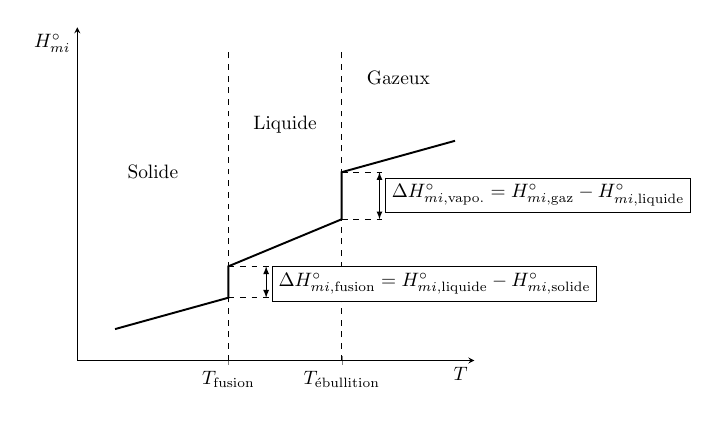
\begin{tikzpicture}[scale=0.7]
\begin{axis}[
    clip = false,
    axis lines = left,
    axis line style={shorten >=-10pt},
    xlabel={$T$}, ylabel={$H_{mi}^\circ$},
    xmax=5, ymax=5, xmin=0, ymin=0,
    xtick={2,3.5},
    xticklabels={$T_{\mathrm{fusion}}$,$T_{\acute{\mathrm{e}}\mathrm{bullition}}$, $T_2$},
    ytick=\empty,
    every axis x label/.style={anchor=north east,at={(1,0)},xshift=10pt}, every axis y label/.style={anchor=north east,at={(0,1)},yshift=10pt}, >=latex]

% grille au cas-où
%\draw[step=0.5,gray!50,very thin] (0,0) grid (5,5);

% Courbe
\addplot[no markers,color=black,style=solid,line width=1pt] coordinates {(0.5,0.5) (2,1) (2,1.5) (3.5,2.25) (3.5,3) (5,3.5)};

% pointillés température
\draw [dashed] (2,0) -- (2,5);
\draw [dashed] (3.5,0) -- (3.5,5);

%pointillés ordonnés
\draw [dashed] (2,1) -- (2.6,1);
\draw [dashed] (2,1.5) -- (2.6,1.5);
\draw [dashed] (3.5,2.25) -- (4.1,2.25);
\draw [dashed] (3.5,3) -- (4.1,3);

%flèches verticales
\draw [<->] (2.5,1) -- (2.5,1.5) node [anchor=north west, xshift=1mm, draw=black, fill=white]{$\Delta H^\circ_{mi,\mathrm{fusion}} = H^\circ_{mi,\mathrm{liquide}}- H^\circ_{mi,\mathrm{solide}}$};
\draw [<->] (4,2.25) -- (4,3) node [anchor= north west, yshift=-1mm, xshift=1mm, draw=black, fill=white]{$\Delta H^\circ_{mi,\mathrm{vapo.}} = H^\circ_{mi,\mathrm{gaz}}- H^\circ_{mi,\mathrm{liquide}}$};

% Phases
\node at (1,3) {Solide};
\node at (2.75,3.75) {Liquide};
\node at (4.25,4.5) {Gazeux};

\end{axis}
\end{tikzpicture}
\caption*{L'enthalpie standard de vaporisation est plus grande que celle fusion ($\SI{4e1}{\kilo\joule\per\mole}$ contre $\SI{6}{\kilo\joule\per\mole}$ pour l’eau)}
\end{subfigure}
\hfill
\begin{subfigure}[t]{0.5\textwidth}

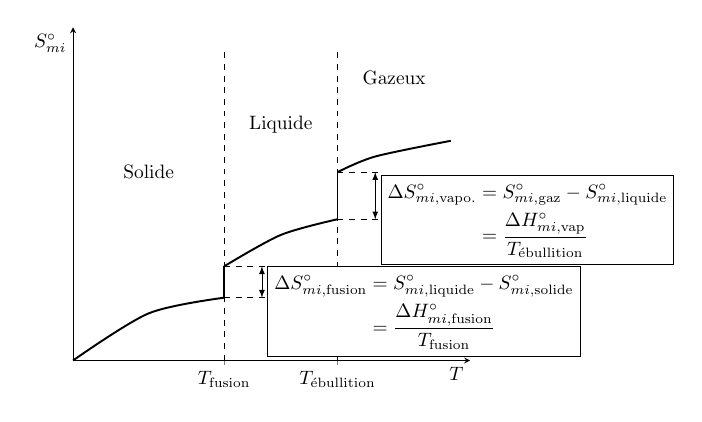
\begin{tikzpicture}[scale=0.7]
\begin{axis}[clip = false, axis lines = left, axis line style={shorten >=-10pt}, xlabel={$T$}, ylabel={$S_{mi}^\circ$}, xmax=5, ymax=5, xmin=0, ymin=0, xtick={2,3.5}, xticklabels={$T_{\mathrm{fusion}}$,$T_{\acute{\mathrm{e}}\mathrm{bullition}}$, $T_2$}, ytick=\empty, every axis x label/.style={anchor=north east,at={(1,0)},xshift=10pt}, every axis y label/.style={anchor=north east,at={(0,1)},yshift=10pt}, >=latex]

% grille au cas-où
%\draw[step=0.5,gray!50,very thin] (0,0) grid (5,5);

% Courbe
\addplot[smooth, no markers,color=black,style=solid,line width=1pt] coordinates {(0,0) (1,0.75) (2,1)};
\addplot[no markers,color=black,style=solid,line width=1pt] coordinates {(2,1) (2,1.5)};
\addplot[smooth, no markers,color=black,style=solid,line width=1pt] coordinates {(2,1.5) (2.75,2) (3.5,2.25)};
\addplot[no markers,color=black,style=solid,line width=1pt] coordinates {(3.5,2.25) (3.5,3)};
\addplot[smooth, no markers,color=black,style=solid,line width=1pt] coordinates {(3.5,3) (4,3.25) (5,3.5)};

% pointillés température
\draw [dashed] (2,0) -- (2,5);
\draw [dashed] (3.5,0) -- (3.5,5);

%pointillés horizontaux
\draw [dashed] (2,1) -- (2.6,1);
\draw [dashed] (2,1.5) -- (2.6,1.5);
\draw [dashed] (3.5,2.25) -- (4.1,2.25);
\draw [dashed] (3.5,3) -- (4.1,3);

\draw [<->] (4,2.25) -- (4,3) node [anchor= north west, yshift=-0.5mm, xshift=1mm, fill=white, draw=black]{$\begin{aligned}\Delta S^\circ_{mi,\mathrm{vapo.}} &= S^\circ_{mi,\mathrm{gaz}}- S^\circ_{mi,\mathrm{liquide}}\\&=\frac{\Delta H^\circ_{mi,\mathrm{vap}} }{T_{\acute{\mathrm{e}}\mathrm{bullition}}}\end{aligned}$};
\draw [<->] (2.5,1) -- (2.5,1.5) node [anchor=north west,xshift=1mm, fill=white, draw=black]{$\begin{aligned}\Delta S^\circ_{mi,\mathrm{fusion}} &= S^\circ_{mi,\mathrm{liquide}}- S^\circ_{mi,\mathrm{solide}}\\&=\frac{\Delta H^\circ_{mi,\mathrm{fusion}} }{T_{\mathrm{fusion}}}\end{aligned}$};


% Phases
\node [align=center,fill=white] at (1,3){Solide};
\node [align=center,fill=white] at (2.75,3.75){Liquide};
\node [align=center,fill=white] at (4.25,4.5){Gazeux};

\end{axis}
\end{tikzpicture}
\end{subfigure}
\end{figure}



\subsection*{Annexe n°3~: Un peu d’histoire des sciences, qui étaient-ils~?}
\begin{multicols*}{4}


Gustav Robert Kirchhoff (1824, Königsberg, 1887, Berlin), Physicien allemand, de tout premier plan, célèbre pour l'énoncé des lois des mailles en électrocinétique. 
On lui doit aussi quelques contributions en thermo-dynamique (le modèle du corps noir) et en électromagnétisme en établissant une théorie scalaire de la diffraction plus générale que le principe de Huygens-Fresnel.
\begin{Figure}
    \centering
    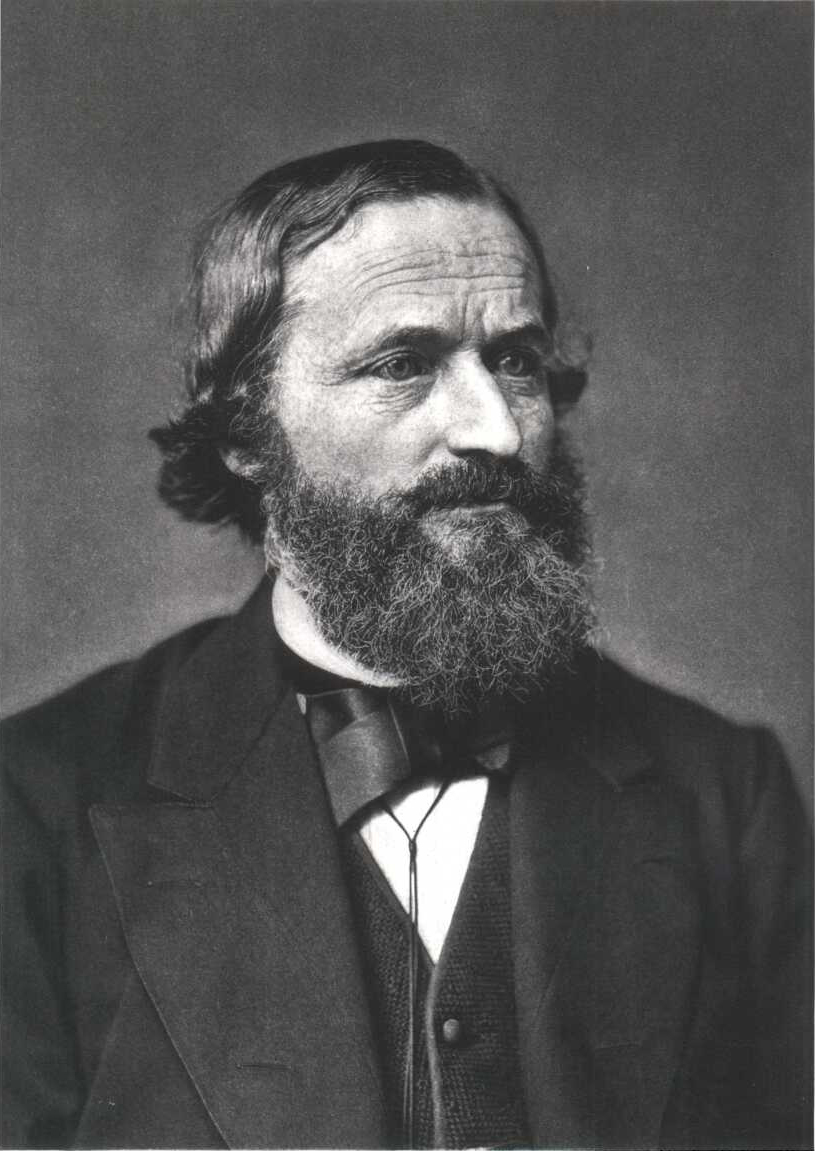
\includegraphics[width=4cm]{ressources/Gustav_Robert_Kirchhoff.jpg}
    \captionof*{figure}{Gustav \textsc{Kirchhoff}}
\end{Figure}
\columnbreak

Jacobus Hendrikus Van’t Hoff (1852 – 1911) est un chimiste néerlandais à la houppette éventée. Il a reçu le premier prix Nobel de chimie en 1901 pour ses travaux décisifs chez Loréal ® sur les laques stabilisatrices des houppettes (parce qu’il le valait bien~!). Plus sérieusement, ses principaux travaux de recherche en chimie fondamentale ont concerné la caractérisation des équilibres chimiques en thermodynamique et des vitesses de réaction en cinétique chimique (loi cinétique de Van’t Hoff).
\begin{Figure}
    \centering
    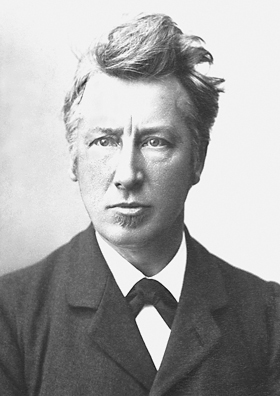
\includegraphics[width=4cm]{ressources/Vant_Hoff.jpg}
    \captionof*{figure}{Jacobus \textsc{Van't Hoff}}
\end{Figure}
\end{multicols*}




\begin{wrapfigure}{r}{4cm}
    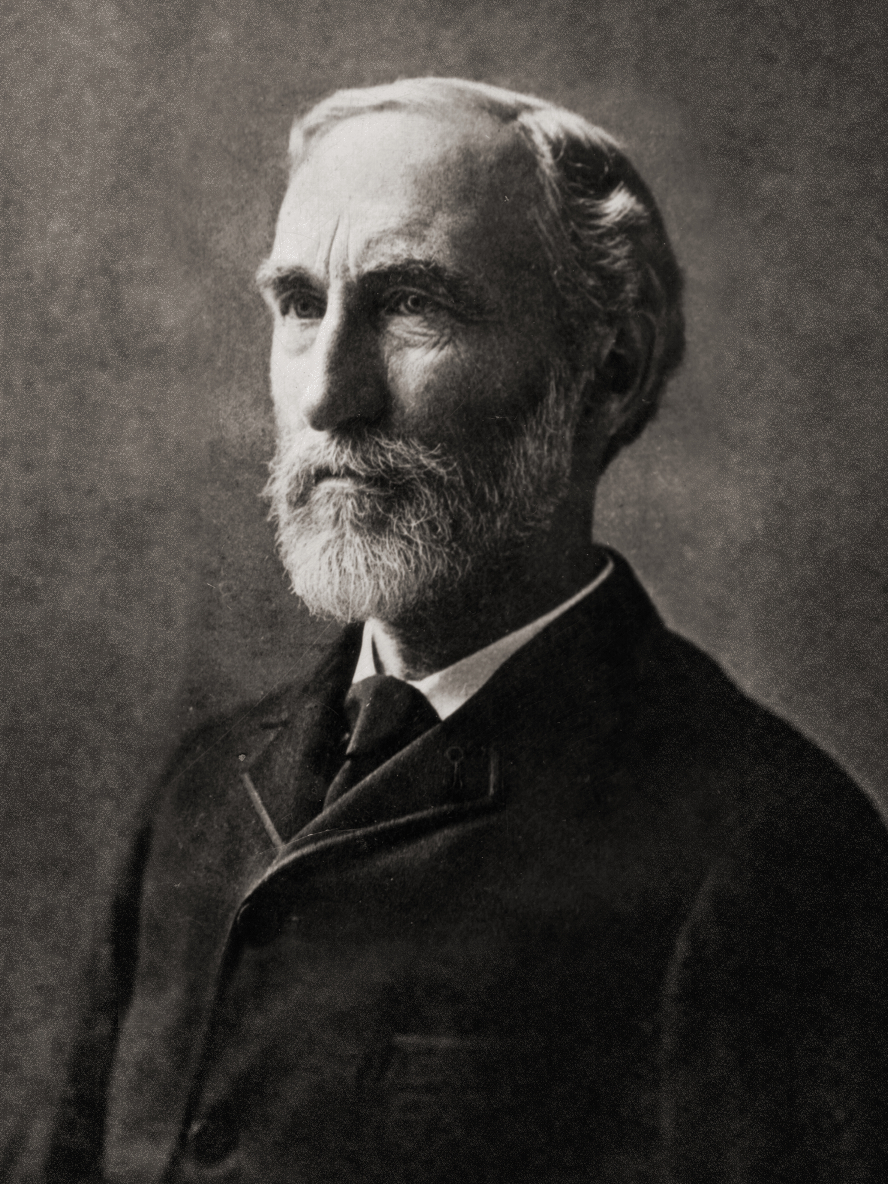
\includegraphics[width=4cm]{ressources/Josiah_Willard_Gibbs.jpg}
    \caption*{Josiah Willard \textsc{Gibbs}}
\end{wrapfigure}
Josiah Willard Gibbs (1839 – 1903), physicien et chimiste américain. Il fut  l’auteur de travaux décisifs en thermodynamique chimique et en physique statistique. Il publia dans les années 1870 une série d’articles sous le titre \textit{On the equilibrium of heterogeneous substances}, qui constituent la base de la thermodynamique chimique~; il y introduit les notions de potentiel chimique, d’enthalpie libre et de variance (« règle des phases » de Gibbs). Ses travaux, publiés dans une revue confidentielle, restèrent dans l’ombre pendant une vingtaine d’années, jusqu’à leur traduction en allemand et en français. Les réactions chimiques se faisant usuellement en contact avec l’atmosphère, elles sont monothermes et monobares~: l’enthalpie libre $G$ est la fonction thermodynamique de la chimie.

\vspace{0.75cm}
\subsection*{Annexe n°4~: Tableau récapitulatif de l’expression du potentiel chimique}
\vspace{-0.1cm}
\begin{table}[H]
\centering
\begin{tabular}{|c|c|c|c|}
   \hline
    \textbf{Hypothèse} & \makecell{\textbf{Activité du}\\\textbf{constituant $B_i$}} & \makecell{\textbf{Commentaire (en}\\\textbf{français dans le texte)}} & \makecell{\textbf{Expression du potentiel}\\\textbf{chimique}}\\
    \hline
    \makecell{Gaz parfait pur\\sous la pression $P$} & $\ds a_i = \frac{P^*}{P^\circ}$ & \makecell{Rapport de la pression\\du gaz pur à la\\ pression de référence\\$\Pz$} & $\ds\mu^*(T,P) = \mu^\circ(T) + RT\ln\bigg(\frac{P^\star}{P^\circ}\bigg)$\\
    \hline
    \makecell{Constituant $B_i$\\d'un mélange idéal\\de gaz parfaits} & $\ds a_i = \frac{P_i}{P^\circ}$ & \makecell{Rapport de la pression\\partielle du\\constituant $B_i$ gazeux\\à la pression de\\référence $\Pz$} & $\ds\mu^*(T,P,n_i) = \mu_i^\circ(T) + RT\ln\bigg(\frac{P_i}{P^\circ}\bigg)$\\
    \hline
    \makecell{Corps pur condensé\\(liquide pur ou\\solide pur)} & $\ds a_i = 1$ & \makecell{La valeur de $1$ est rigou-\\reuse si $\Pz$~;\\elle n'est qu'approchée\\si $P\neq P^\circ$} & $\ds\mu^*(T,P,n_i) = \mu^\circ(T)$\\
    \hline
    \makecell{Constituant $B_i$\\d'un mélange\\condensé idéal} & $\ds a_i = x_i$ & \makecell{Fraction molaire du\\constituant $B_i$ dans\\le mélange} & $\ds\mu(T,n_i) = \mu_i^\circ(T) + RT\ln(x_i)$\\
    \hline
    Solvant & $a_i=1$ & $1$ & $\mu(T) = \mu^\circ(T)$\\
    \hline
    \makecell{Soluté\\(solution idéale)} & $\ds a_i = \frac{c_i}{c^\circ}$ & \makecell{Rapport de la\\concentration du\\soluté à la concen-\\tration de référence\\$\cz$} & $\ds\mu(T,c_i) = \mu_i^\circ(T) + RT\ln\bigg(\frac{c_i}{c^\circ}\bigg)$\\
    \hline
\end{tabular}
\end{table}
\end{document}